\documentclass{beamer}

\pdfmapfile{+sansmathaccent.map}


\mode<presentation>
{
	\usetheme{Warsaw} % or try Darmstadt, Madrid, Warsaw, Rochester, CambridgeUS, ...
	\usecolortheme{seahorse} % or try seahorse, beaver, crane, wolverine, ...
	\usefonttheme{serif}  % or try serif, structurebold, ...
	\setbeamertemplate{navigation symbols}{}
	\setbeamertemplate{caption}[numbered]
} 


%%%%%%%%%%%%%%%%%%%%%%%%%%%%
% itemize settings


%%%%%%%%%%%%%%%%%%%%%%%%%%%%
% itemize settings

\definecolor{myhotpink}{RGB}{255, 80, 200}
\definecolor{mywarmpink}{RGB}{255, 60, 160}
\definecolor{mylightpink}{RGB}{255, 80, 200}
\definecolor{mypink}{RGB}{255, 30, 80}
\definecolor{mydarkpink}{RGB}{155, 25, 60}

\definecolor{mypaleblue}{RGB}{240, 240, 255}
\definecolor{mylightblue}{RGB}{120, 150, 255}
\definecolor{myblue}{RGB}{90, 90, 255}
\definecolor{mygblue}{RGB}{70, 110, 240}
\definecolor{mydarkblue}{RGB}{0, 0, 180}
\definecolor{myblackblue}{RGB}{40, 40, 120}

\definecolor{myblackturquoise}{RGB}{5, 53, 60}
\definecolor{mydarkdarkturquoise}{RGB}{8, 93, 110}
\definecolor{mydarkturquoise}{RGB}{28, 143, 150}
\definecolor{mypaleturquoise}{RGB}{230, 255, 255}
\definecolor{myturquoise}{RGB}{48, 213, 200}

\definecolor{mygreen}{RGB}{0, 200, 0}
\definecolor{mydarkgreen}{RGB}{0, 120, 0}
\definecolor{mygreen2}{RGB}{245, 255, 230}

\definecolor{mygrey}{RGB}{120, 120, 120}
\definecolor{mypalegrey}{RGB}{160, 160, 160}
\definecolor{mydarkgrey}{RGB}{80, 80, 160}

\definecolor{mydarkred}{RGB}{160, 30, 30}
\definecolor{mylightred}{RGB}{255, 150, 150}
\definecolor{myred}{RGB}{200, 110, 110}
\definecolor{myblackred}{RGB}{120, 40, 40}

\definecolor{mygreen}{RGB}{0, 200, 0}
\definecolor{mygreen2}{RGB}{205, 255, 200}

\definecolor{mydarkcolor}{RGB}{60, 25, 155}
\definecolor{mylightcolor}{RGB}{130, 180, 250}

\setbeamertemplate{itemize items}[default]

\setbeamertemplate{itemize item}{\color{myblackturquoise}$\blacksquare$}
\setbeamertemplate{itemize subitem}{\color{mydarkdarkturquoise}$\blacktriangleright$}
\setbeamertemplate{itemize subsubitem}{\color{mygray}$\blacksquare$}

\setbeamercolor{palette quaternary}{fg=white,bg=myblackturquoise}
\setbeamercolor{titlelike}{parent=palette quaternary}

\setbeamercolor{palette quaternary2}{fg=black,bg=mypaleblue}
\setbeamercolor{frametitle}{parent=palette quaternary2}

\setbeamerfont{frametitle}{size=\Large,series=\scshape}
\setbeamerfont{framesubtitle}{size=\normalsize,series=\upshape}





%%%%%%%%%%%%%%%%%%%%%%%%%%%%
% block settings

\setbeamercolor{block title}{bg=red!30,fg=black}

\setbeamercolor*{block title example}{bg=mygreen!40!white,fg=black}

\setbeamercolor*{block body example}{fg= black, bg= mygreen2}


%%%%%%%%%%%%%%%%%%%%%%%%%%%%
% URL settings
\hypersetup{
	colorlinks=true,
	linkcolor=blue,
	filecolor=blue,      
	urlcolor=blue,
}

%%%%%%%%%%%%%%%%%%%%%%%%%%

\renewcommand{\familydefault}{\rmdefault}

\usepackage{amsmath}
\usepackage{mathtools}

\usepackage{subcaption}

\usepackage{qrcode}

\DeclareMathOperator*{\argmin}{arg\,min}
\newcommand{\bo}[1] {\mathbf{#1}}

\newcommand{\R}{\mathbb{R}} 
\newcommand{\T}{^\top}     



\newcommand{\mydate}{Fall 2023}

\newcommand{\mygit}{\textcolor{blue}{\href{https://github.com/SergeiSa/Control-Theory-Slides-Spring-2023}{github.com/SergeiSa/Control-Theory-Slides-Spring-2023}}}

\newcommand{\myqr}{ \textcolor{black}{\qrcode[height=1.5in]{https://github.com/SergeiSa/Control-Theory-Slides-Spring-2023}}
}

\newcommand{\myqrframe}{
	\begin{frame}
		\centerline{Lecture slides are available via Github, links are on Moodle}
		\bigskip
		\centerline{You can help improve these slides at:}
		\centerline{\mygit}
		\bigskip
		\myqr
	\end{frame}
}


\newcommand{\bref}[2] {\textcolor{blue}{\href{#1}{#2}}}

%%%%%%%%%%%%%%%%%%%%%%%%%%%%
% code settings

\usepackage{listings}
\usepackage{color}
% \definecolor{mygreen}{rgb}{0,0.6,0}
% \definecolor{mygray}{rgb}{0.5,0.5,0.5}
\definecolor{mymauve}{rgb}{0.58,0,0.82}
\lstset{ 
	backgroundcolor=\color{white},   % choose the background color; you must add \usepackage{color} or \usepackage{xcolor}; should come as last argument
	basicstyle=\footnotesize,        % the size of the fonts that are used for the code
	breakatwhitespace=false,         % sets if automatic breaks should only happen at whitespace
	breaklines=true,                 % sets automatic line breaking
	captionpos=b,                    % sets the caption-position to bottom
	commentstyle=\color{mygreen},    % comment style
	deletekeywords={...},            % if you want to delete keywords from the given language
	escapeinside={\%*}{*)},          % if you want to add LaTeX within your code
	extendedchars=true,              % lets you use non-ASCII characters; for 8-bits encodings only, does not work with UTF-8
	firstnumber=0000,                % start line enumeration with line 0000
	frame=single,	                   % adds a frame around the code
	keepspaces=true,                 % keeps spaces in text, useful for keeping indentation of code (possibly needs columns=flexible)
	keywordstyle=\color{blue},       % keyword style
	language=Octave,                 % the language of the code
	morekeywords={*,...},            % if you want to add more keywords to the set
	numbers=left,                    % where to put the line-numbers; possible values are (none, left, right)
	numbersep=5pt,                   % how far the line-numbers are from the code
	numberstyle=\tiny\color{mygray}, % the style that is used for the line-numbers
	rulecolor=\color{black},         % if not set, the frame-color may be changed on line-breaks within not-black text (e.g. comments (green here))
	showspaces=false,                % show spaces everywhere adding particular underscores; it overrides 'showstringspaces'
	showstringspaces=false,          % underline spaces within strings only
	showtabs=false,                  % show tabs within strings adding particular underscores
	stepnumber=2,                    % the step between two line-numbers. If it's 1, each line will be numbered
	stringstyle=\color{mymauve},     % string literal style
	tabsize=2,	                   % sets default tabsize to 2 spaces
	title=\lstname                   % show the filename of files included with \lstinputlisting; also try caption instead of title
}


%%%%%%%%%%%%%%%%%%%%%%%%%%%%
% URL settings
\hypersetup{
	colorlinks=false,
	linkcolor=blue,
	filecolor=blue,      
	urlcolor=blue,
}

%%%%%%%%%%%%%%%%%%%%%%%%%%

%%%%%%%%%%%%%%%%%%%%%%%%%%%%
% tikz settings

\usepackage{tikz}
\tikzset{every picture/.style={line width=0.75pt}}


\title{Second order systems}
\subtitle{Mechatronics, Lecture 6}
\author{by Sergei Savin}
\centering
\date{\mydate}



\begin{document}
\maketitle



\begin{frame}{Content}
\begin{itemize}
\item Steady State
%\item Static State
%\item Power
%\item Efficiency
%\item Static power
%\item Reducer and power
\end{itemize}
\end{frame}





\begin{frame}{Second-order systems}
	% \framesubtitle{O}
	\begin{flushleft}
		
		Some of the second-order dynamical systems we have seen before:
		
		\begin{itemize}
			\item Spring-mass-damper dynamics.
			\item RLC circuit.
			\item DC motor angular velocity dynamics.
			\item Linearized model of a pendulum.
		\end{itemize}
	
		In a few lectures we will see that PID controller also acts in a way similar to a second-order dynamical system.
		
		\bigskip
		
		Since any polynomial can be represented as a product of linear polynomials and quadratic polynomials, we can also re-write any transfer function as a product of transfer functions with quadratic polynomials in the denominator. We can see second-order dynamical systems as fundamental building blocks of dynamical systems.
		
	\end{flushleft}
\end{frame}



\begin{frame}{Eigenvalues, 1}
	% \framesubtitle{O}
	\begin{flushleft}
		
		Observing eq. $m \ddot y + \mu_0 \dot y + c_0 y = 0$ we can tell that it is stable if (sufficient but not necessary condition) $m > 0$, $\mu > 0$, and $c > 0$ - this follows from the physics of the system.
		
		\bigskip
		
		A more principled approach is to find eigenvalues of the linear system. We start by dividing the equation by $m$:
		
		\begin{equation}
			\ddot y + \mu \dot y + c y = 0
		\end{equation}
		
		where $\mu = \mu_0 / m$ and $c = c_0 / m$. Defining $x_1 = y$ and $x_2 = \dot y$, the system can be equivalently represented as:
		
		\begin{equation}
			\begin{bmatrix}
				\dot x_1 \\ \dot x_2
			\end{bmatrix}
			=
			\begin{bmatrix}
				0 & 1 \\
				-c & -\mu
			\end{bmatrix} 
			\begin{bmatrix}
				x_1 \\ x_2
			\end{bmatrix}   
		\end{equation}
		
		
	\end{flushleft}
\end{frame}



\begin{frame}{Eigenvalues, 2}
	% \framesubtitle{O}
	\begin{flushleft}
		
		With linear system 
		$
		\begin{bmatrix}
			\dot x_1 \\ \dot x_2
		\end{bmatrix}
		=
		\begin{bmatrix}
			0 & 1 \\
			-c & -\mu
		\end{bmatrix} 
		\begin{bmatrix}
			x_1 \\ x_2
		\end{bmatrix}   
		$, we need to find its eigenvalues. We know that there is a formula for eigenvalues based on trace and determinant:
		
		\begin{equation}
			\lambda = \frac{T \pm \sqrt{T^2 - 4D} }{2}
		\end{equation}
		
		where $T$ is trace and $D$ is the determinant.
		
		\bigskip
		
		In our case $T = -\mu$ and $D = c$, and eigenvalues are:
		
		\begin{equation}
			\lambda = \frac{-\mu \pm \sqrt{\mu^2 - 4c} }{2}
		\end{equation}
		
		
	\end{flushleft}
\end{frame}



\begin{frame}{Eigenvalues, 3}
	% \framesubtitle{O}
	\begin{flushleft}
		
		Lets analyze eigenvalues $\lambda = \frac{-\mu \pm \sqrt{\mu^2 - 4c} }{2}$. We can see that if $\mu \geq 0$ and $c \geq 0$, there are only two scenarios: 
		
		\begin{enumerate}
			\item $\mu^2 - 4c \geq 0$, in which case $\sqrt{\mu^2 - 4c} \leq \mu$, the eigenvalues are purely real and negative.
			\item $\mu^2 - 4c < 0$, in which case $\sqrt{\mu^2 - 4c}$ is a purely imaginary number, the eigenvalues are complex with negative real parts.
		\end{enumerate}
		
		If $\mu \geq 0$ and $c = 0$, $\lambda_1 = -\mu$, $\lambda_2 = 0$, hence the system is marginally stable.
		
	\end{flushleft}
\end{frame}



\begin{frame}{Eigenvalues, 4}
	% \framesubtitle{O}
	\begin{flushleft}
		
		
		If $\mu \geq 0$ and $c < 0$, then $\sqrt{\mu^2 - 4c} \geq \mu$, and eigenvalues are purely real and one of them is positive, the system is unstable. If $\mu < 0$ and $c < 0$ at least one of the eigenvalues is still positive.
		
		\bigskip
		
		If $\mu < 0$ and $c \geq 0$, then again there are only two scenarios: 
		
		\begin{enumerate}
			\item $\mu^2 - 4c \geq 0$, in which case $\sqrt{\mu^2 - 4c} \leq \mu$, the eigenvalues are purely real and positive.
			\item $\mu^2 - 4c < 0$, in which case $\sqrt{\mu^2 - 4c}$ is a purely imaginary number, the eigenvalues are complex with positive real parts.
		\end{enumerate}
		
		\begin{definition}
			If $\mu \geq 0$ and $c \geq 0$ the system is stable, if $\mu < 0$ or $c < 0$ it is unstable.
		\end{definition}
		
	\end{flushleft}
\end{frame}




\begin{frame}{Characteristic polynomial}
	% \framesubtitle{O}
	\begin{flushleft}
		
		Going back to the eq. $\ddot y + \mu \dot y + c y = 0$ we can write characteristic eq. for it:
		
		\begin{equation}
			k^2 y + \mu k + c = 0
		\end{equation}
		
		Its roots are given by the formula:
		
		\begin{equation}
			k = \frac{-\mu \pm \sqrt{\mu^2 - 4c} }{2}
		\end{equation}
		
		As we can see, it is exactly the same as the determinant-trace formula.
		
		
	\end{flushleft}
\end{frame}



\begin{frame}{Transfer function poles}
	% \framesubtitle{O}
	\begin{flushleft}
		
		Now, lets consider the transfer function:
		
		\begin{equation}
			W(s) = \frac{1}{s^2 + \mu s + c }
		\end{equation}
		
		Poles of the transfer functions are solutions of the polynomial in its denominator; notice that this polynomial is exactly the same as the previously discussed characteristic polynomial. Meaning the poles of the transfer function are eigenvalues of the linear system.
		
		
	\end{flushleft}
\end{frame}



\begin{frame}{Natural frequency representation, 1}
	% \framesubtitle{O}
	\begin{flushleft}
		
		Another popular form of writing a second-order ODE is the following:
		
		\begin{equation}
			\ddot y + 2 \zeta \omega_n \dot y + \omega_n^2 y = 0
		\end{equation}
		%
		where $\omega_n$ is a \emph{natural frequency} and $\zeta$ is \emph{damping factor}. The quantity $\zeta \omega_n$ is called \emph{damping attenuation}. The relation between $\zeta, \omega_n$ and $\mu, c$ is:
		
		\begin{align}
			\omega_n = \sqrt{c},  \ \ \ \ \zeta = \frac{\mu}{2\sqrt{c}}
		\end{align}
	
		With this, the expression for eigenvalues is:
		
		\begin{equation}
			\lambda = -\zeta \omega_n \pm \omega_n \sqrt{\zeta^2 - 1}
		\end{equation}
		
	\end{flushleft}
\end{frame}


\begin{frame}{Natural frequency representation, 2}
	% \framesubtitle{O}
	\begin{flushleft}
		
		With the representation $\ddot y + 2 \zeta \omega_n \dot y + \omega_n^2 y = 0$ we can tell:
		
		\bigskip
		
		\begin{itemize}
			\item the system is overdamped (has pure real negative eigenvalues) is $\zeta > 1$, critically damped if $\zeta = 1$ and underdamped (produces oscillations) if  $0 \leq \zeta<1$;
			
			\item the system has purely imaginary eigenvalues (non-decaying oscillations) iff $\zeta = 0$ (since $\omega_n = 0$ corresponds to the trivial solution).
		\end{itemize}
		
		 
	\end{flushleft}
\end{frame}




\begin{frame}{Natural frequency representation, 3}
	% \framesubtitle{O}
	\begin{flushleft}
		
		\begin{figure}
			\centering
			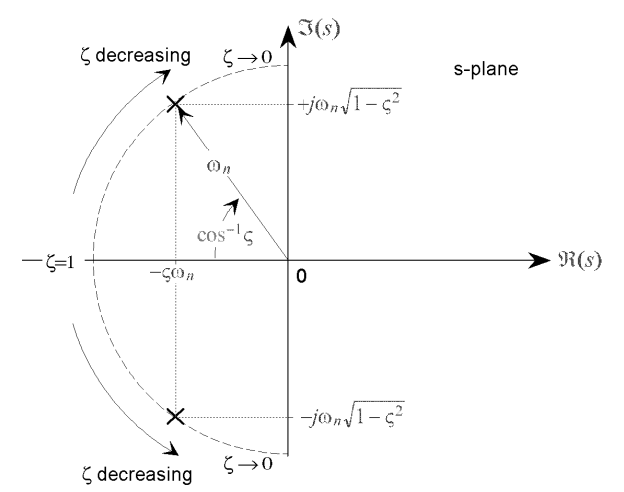
\includegraphics[width=0.8\linewidth]{Poles}
			\caption{Poles and $\zeta, \omega_n$. \bref{https://web.mit.edu/2.14/www/Handouts/PoleZero.pdf}{Credit: MIT}.}
		\end{figure}
		
	\end{flushleft}
\end{frame}



\begin{frame}{Pure imaginary poles, 1}
	% \framesubtitle{O}
	\begin{flushleft}
		
		Given $\zeta = 0$ (implying $\mu = 0$) we have pure imaginary poles / eigenvalues $\lambda = \pm i \omega_n$. Moreover, the dynamics equations become:
		
		\begin{equation}
			\ddot y + \omega_n^2 y = 0
		\end{equation}
		
		Proposing solution $y = A \sin (\omega_n t + \varphi)$, noting that $\dot y = \omega_n A \cos (\omega_n t + \varphi)$ and $\ddot y = -\omega_n^2 A\sin (\omega_n t + \varphi)$, we see:
		
		\begin{align}
			-\omega_n^2 A\sin (\omega_n t + \varphi) + \omega_n^2 A \sin (\omega_n t + \varphi) = 0
		\end{align}
		%
		which is an equality.
		
		
	\end{flushleft}
\end{frame}




\begin{frame}{Pure imaginary poles, 2}
	% \framesubtitle{O}
	\begin{flushleft}
		
		Previous slide showed that the system without damping $\ddot y + \omega_n^2 y = 0$ will oscillate with angular frequency $\omega_n$; this motivates the name "natural frequency".
		
		\bigskip
		
		Also it shows that, if we pass a harmonic signal with angular frequency $\omega_n$ through a transfer function $W(s) = s^2 + \omega_n^2$ we will get a zero output.
		
		\bigskip
		
		Alternately, passing a harmonic signal with angular frequency $\omega_n$ through a transfer function $W(s) = \frac{1}{s^2 + \omega_n^2}$ we observe an infinite gain. Same can be observed by substituting $i \omega$ for $s$ and evaluating the absolute value of the transfer function at $\omega = \omega_n$. This effect is called \emph{resonance}.
		
		
	\end{flushleft}
\end{frame}




\begin{frame}{Frequency response}
	% \framesubtitle{O}
	\begin{flushleft}
		
		Given a transfer function $W(s) = \frac{1}{s^2 + 2 \zeta \omega_n s + \omega_n^2}$ we can find frequency response gain by computing absolute value of $W(i\omega)$:
		
		\begin{equation}
			G = |W(i\omega)| = \frac{1}{\sqrt{(\omega_n^2 - \omega^2)^2 + (2 \zeta \omega_n \omega)^2}}
		\end{equation}
	
	\begin{itemize}
		\item As $\omega \rightarrow 0$, $G \rightarrow \frac{1}{\omega_n^2}$.
		\item As $\omega \rightarrow \omega_n$, $G \rightarrow \frac{1}{\sqrt{2\zeta}\omega_n^2}$.
		\item As $\omega \rightarrow \infty$, $G \rightarrow 0$.
	\end{itemize}
		
		
	\end{flushleft}
\end{frame}



\begin{frame}{Read more}
	% \framesubtitle{Local coordinates}
	\begin{flushleft}
		
		\begin{itemize}
			\item \bref{https://web.mit.edu/2.14/www/Handouts/PoleZero.pdf}{MIT. 2.14 Analysis and Design of Feedback Control Systems. Understanding Poles and Zeros}
			
		\end{itemize}
		
		
	\end{flushleft}
\end{frame}


\myqrframe

\end{document}
